%\section{Training a Sentence Classifier without Alignment \label{sec:uschema}}
\section{Model \label{sec:model}}

\subsection {Universal Schema without Entity Embeddings}

While Compositional Universal Schema addresses reasoning over arbitrary textual patterns, it is still limited to reasoning over entity pairs seen at training time.
\citet{verga2015multilingual} approach this problem by using Universal Schema as a sentence classifier - directly comparing a textual relation to a kb relation to perform relation extraction.
However, this approach is unsatisfactory for two reasons.
The first is that this creates an inconsistency between training and testing, as the model is trained to predict compatibality between entity pairs and relations and not relations directly.
Secondly, it considers only a single piece of evidence while making its prediction.
The learned entity pair can be seen as a sumamrization of all relations for which that entity pair was seen.
Because of this, it should be possible to reconstruct an entity pair representation from its relation types.
%\todo{describe that its uscham + aggregation - refer to figures}



\begin{figure}[h]
\caption{Aggragating relation type vectors to form entity pair vector}
\centering
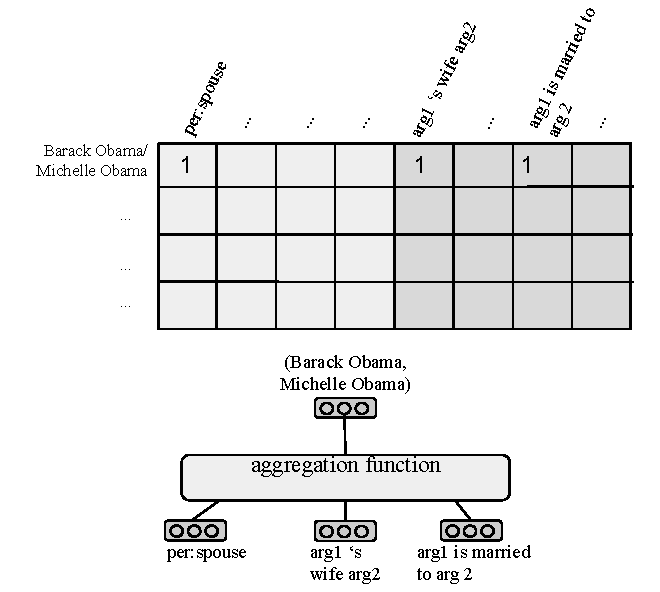
\includegraphics[scale=.68]{aggregate-entity}
\end{figure}


\subsection {Aggregation Functions \label{sec:functions}}
In this work we examine several fairly simple aggregation functions.
\textbf{Mean Relation} creates a single centroid for the entity pair by averaging all of its relation vectors.
While this intuitive makes sense as an approximation for the explicit entity pair representation, averaging large numbers of embeddings can lead to a noisy signal.
The \textbf{Max Relation} represents the entity pair as its most similar relation to the query vector of interest.
This model has the advantage of creating a query specific entity pair representation but also is more susceptible to noisey training data as a single incorrect piece of evidence could be used to form a prediction.
\textbf {TopK Relations} is a middle ground between Mean and Max relations.
Finally, we look at dimension-wise \textbf{Max Pool}.
Like Mean Relation, this allows the model to pool relevant information over the entire set of relations.

\subsection {Training}
Training the standard Universal Schema model is performed using Bayesian Personalized Ranking (BPR)~\citep{rendle2009bpr} which seeks to rank the probability of observed triples above unobserved triples rather than explicitly model unobserved edges as negative.
Each training example is an entity pair/relation type triple observed in the training text corpora or KB.

Our training procedure for our relation-only Universal Schema model is very similar to the original model.
We first pool all of the observed triples in our training data by entity pair creating entity pair specific relation sets $R^{Ep}$.
We then construct training examples for each observed relation type of an entity and an aggregation of all other relation types observed with that entity.
For each $r_i \in R^{Ep}$, construct training example $(r_i, \left\{R^{Ep}\setminus r_i\right\})$.
We randomly sample a differnent relation to act as the negative sample.
